\section{Casos de Uso del Usuario}

\subsection{Diagrama de Casos de Uso General del Usuario}

\begin{figure}[htbp]
	\centering
		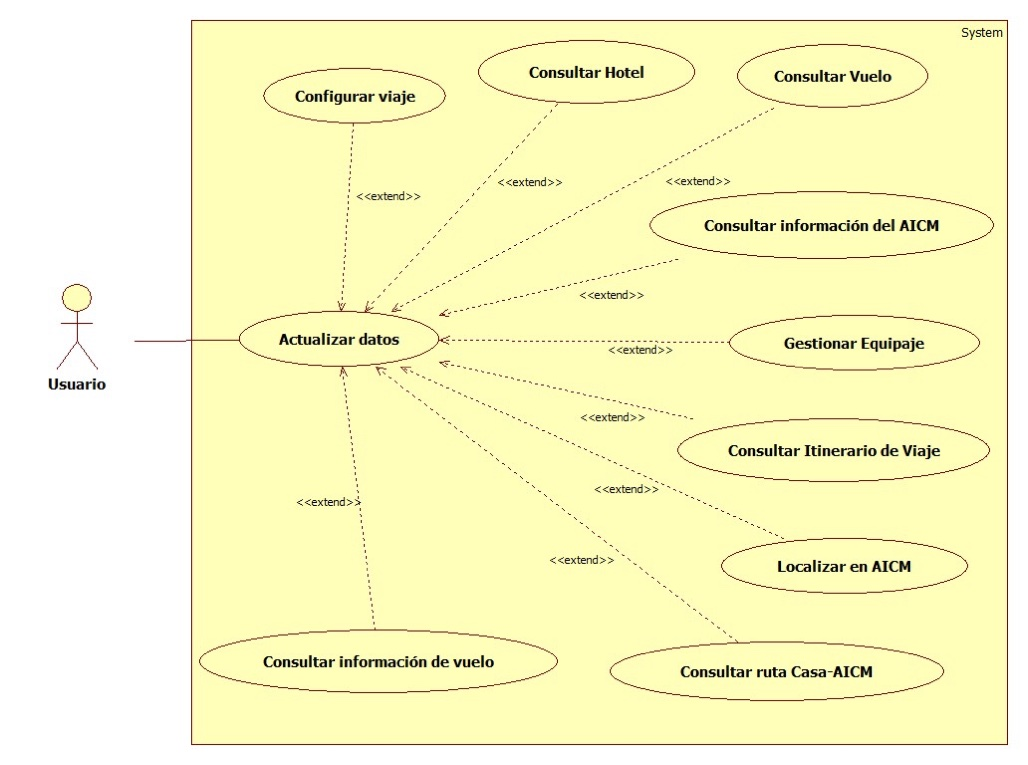
\includegraphics[width=1\textwidth]{Figuras/cugeneralUsuario.jpg}
		\rule{30em}{0.5pt}
	\caption[Diagrama de Casos de Uso General del Usuario]{Diagrama de Casos de Uso General del Usuario}
	\label{fig:cuGeneralUsuario}
\end{figure}
\clearpage

\subsection{Caso de Uso Actualizar Datos}

\begin{figure}[htbp]
	\centering
		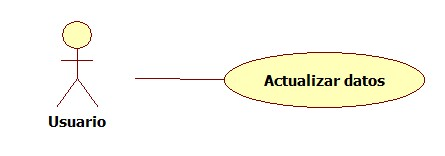
\includegraphics[width=0.9\textwidth]{Figuras/cuActualizarDatos.jpg}
		\rule{30em}{0.5pt}
	\caption[Diagrama de Caso de Uso Actualizar Datos]{Diagrama de Caso de Uso Actualizar Datos}
	\label{fig:cuActualizarDatos}
\end{figure}

\begin{longtable}[h]{|p{2.5cm}|p{6.4cm}|p{2cm}|p{2cm}|}
	\hline
		\rowcolor[RGB]{51,153,255}{Caso de Uso}&\multicolumn{2}{c}{Actualizar Datos}&{\textbf{CU-U-01}}\\
	\hline
		{Actores}&\multicolumn{3}{p{11.2cm}|}{Usuario}\\
	\hline
		{Tipo}&\multicolumn{3}{p{11.2cm}|}{Esencial}\\
	\hline
		{Precondición}&\multicolumn{3}{p{11.2cm}|}{El usuario debe iniciar la aplicación móvil.}\\
	\hline
		{Postcondición}&\multicolumn{3}{p{11.2cm}|}{La base de datos se ha actualizado con la información del servicio web de TASMC y se ha actualizado la última fecha de ingreso a la aplicación móvil TASMC.}\\
	\hline
		{Autor}&{Barajas Uribe Sergio}&{\textbf{Fecha} 05/06/15}&{\textbf{Versión} 1.0}\\
			\hline
		{Evaluador}&{Barajas Uribe Sergio}&{\textbf{Fecha} 07/06/15}&{\textbf{Estatus} Aprobado}\\
	\hline
		{Propósito}&\multicolumn{3}{p{11.2cm}|}{Mantener la información tanto en la aplicación móvil como en el web service TASMC actualizada.}\\
	\hline
		{Resumen}&\multicolumn{3}{p{11.2cm}|}{El sistema hace la petición al web service TASMC de la información sobre la lista de equipaje y actualiza la base de datos de la aplicación móvil. Asimismo, envía la información del usuario que ingresó a la aplicación móvil al web service TASMC para actualizar la fecha de último ingreso.}\\	
	\hline
		{Comentarios}&\multicolumn{3}{p{11.2cm}|}{Este proceso se ejecutará cuando el usuario este conectado a una red vía Wifi}\\	
	\hline
	\caption[Especificación del Caso de Uso Actualizar Datos]{Especificación del Caso de Uso Actualizar Datos}
    	\label{tab:cuActualizarDatos}
\end{longtable}
\newpage
\begin{flushleft}
	\textbf{Trayectoria Principal}\\
	\begin{enumerate}
		\item El sistema hace una petición al web service TASMC para que le envíe la información de las listas de equipaje.
		\item El sistema actualiza la base de datos con la información enviada por el web service TASMC.
		\item El sistema envía la información del usuario al web service TASMC.
		\item El web service TASMC actualiza la fecha de última visita del usuario.
	\end{enumerate}
\end{flushleft}
----Fin del caso de uso
\newpage

\subsection{Caso de Uso Configurar Viaje}

\begin{figure}[htbp]
	\centering
		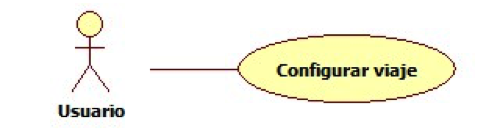
\includegraphics[width=0.9\textwidth]{Figuras/cuConfigurarViaje.png}
		\rule{30em}{0.5pt}
	\caption[Diagrama de Caso de Uso Configurar Viaje]{Diagrama de Caso de Uso Configurar Viaje}
	\label{fig:cuConfigurarViaje}
\end{figure}

\begin{longtable}[h]{|p{2.5cm}|p{6.4cm}|p{2cm}|p{2cm}|}
	\hline
		\rowcolor[RGB]{51,153,255}{Caso de Uso}&\multicolumn{2}{c}{Configurar Viaje}&{\textbf{CU-U-02}}\\
	\hline
		{Actores}&\multicolumn{3}{p{11.2cm}|}{Usuario}\\
	\hline
		{Tipo}&\multicolumn{3}{p{11.2cm}|}{Esencial}\\
	\hline
		{Precondición}&\multicolumn{3}{p{11.2cm}|}{El usuario puede o no realizar su configuración de viaje, pero la aplicación le hará la sugerencia de realizarla en otro momento.}\\
	\hline
		{Postcondición}&\multicolumn{3}{p{11.2cm}|}{La configuración del usuario ha quedado registrada, por lo tanto, está en condiciones de hacer uso de los servicios ofrecidos por el sistema.}\\
	\hline
		{Autor}&{Vivanco Carmona Erick Rafael}&{\textbf{Fecha} 09/01/15}&{\textbf{Versión} 2.0}\\
			\hline
		{Evaluador}&{Barajas Uribe Sergio}&{\textbf{Fecha} 15/01/15}&{\textbf{Estatus} Aprobado}\\
	\hline
		{Propósito}&\multicolumn{3}{p{11.2cm}|}{Configurar sus viajes dependiendo de la clase de viaje que más le agrade al usuario y la categoría de hoteles que frecuenta.}\\
	\hline
		{Resumen}&\multicolumn{3}{p{11.2cm}|}{El usuario realiza la configuración de la aplicación según la clase en la que más le gusta viajar y la categoría de hoteles que desea el usuario además proporciona su correo electrónico para tener el control de su usuario.}\\	
	\hline
		{Comentarios}&\multicolumn{3}{p{11.2cm}|}{Los datos guardados estarán protegidos y únicamente se enviaran notificaciones acerca de la aplicación al correo proporcionado.}\\	
	\hline
	\caption[Especificación del Caso de Uso Configurar Viaje]{Especificación del Caso de Uso Configurar Viaje}
    	\label{tab:cuConfigurarViaje}
\end{longtable}
\newpage
\begin{flushleft}
	\textbf{Trayectoria Principal}\\
	\begin{enumerate}
		\item El usuario inicia la aplicación por primera vez e inmediatamente se le indica si gusta configurar su aplicación con la clase en la que le guste viajar y categoría de hotel que prefiere. \hyperlink{TrayectoriaA_CU-U-02}{[Trayectoria A]}.
		\item El sistema presenta un formulario para que el usuario introduzca su correo electrónico, la clase de viaje y categoría de hotel.
		\item El usuario introduce los datos y los envía para que sean registrados.
		\item El sistema válida la configuración proporcionada por el usuario. \hyperlink{TrayectoriaB_CU-U-02}{[Trayectoria B]}.
		\item La configuración del usuario queda registrada en el sistema. Se notifica al usuario.
	\end{enumerate}
\end{flushleft}
----Fin del caso de uso

\begin{flushleft}
	\hypertarget{TrayectoriaA_CU-U-02}{}
	\textbf{Trayectoria Alternativa A}\\
	\textbf{Condición:} La conexión con el servidor se pierde. \\
	\textbf{Nota: } Este curso alterno puede presentarse en cualquier momento durante el curso de CU-U-02.\\
	\begin{enumerate}
		\item El cliente debe reintentar completar la operación en otro momento. 
		\item Volver a 1. 
	\end{enumerate}
\end{flushleft}
----Fin de Trayectoria

\begin{flushleft}
	\hypertarget{TrayectoriaB_CU-U-02}{}
	\textbf{Trayectoria Alternativa B}\\
	\textbf{Condición:} La configuración no es correcta.  \\
	\begin{enumerate}
		\item Se notifica al usuario y se solicita que los datos erróneos sean modificados. 
		\item Volver a 2.
	\end{enumerate}
\end{flushleft}
----Fin de Trayectoria
\newpage
\subsection{Caso de Uso Consultar Hotel}

\begin{figure}[htbp]
	\centering
		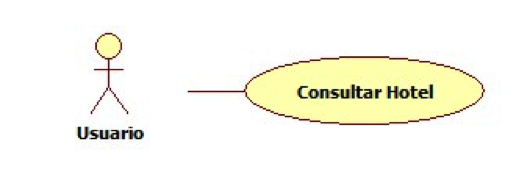
\includegraphics[width=0.9\textwidth]{Figuras/cuConsultarHotel.png}
		\rule{30em}{0.5pt}
	\caption[Diagrama de Caso de Uso Consultar Hotel]{Diagrama de Caso de Uso Consultar Hotel}
	\label{fig:cuConsultarHotel}
\end{figure}

\begin{longtable}{|p{2.5cm}|p{6.4cm}|p{2cm}|p{2cm}|}
	\hline
		\rowcolor[RGB]{51,153,255}{Caso de Uso}&\multicolumn{2}{c}{Consultar Hotel}&{\textbf{CU-U-03}}\\
	\hline
		{Actores}&\multicolumn{3}{p{11.2cm}|}{Usuario}\\
	\hline
		{Tipo}&\multicolumn{3}{p{11.2cm}|}{Esencial}\\
	\hline
		{Precondición}&\multicolumn{3}{p{11.2cm}|}{	Existen hoteles registrados en el Web Service.}\\
	\hline
		{Postcondición}&\multicolumn{3}{p{11.2cm}|}{El turista tiene a su disposición la información de hoteles acorde a sus posibilidades.}\\
	\hline
		{Autor}&{Barajas Uribe Sergio}&{\textbf{Fecha} 06/06/15}&{\textbf{Versión} 3.0}\\
			\hline
		{Evaluador}&{Barajas Uribe Sergio}&{\textbf{Fecha} 07/06/15}&{\textbf{Estatus} Aprobado}\\
	\hline
		{Propósito}&\multicolumn{3}{p{11.2cm}|}{Consultar información de hoteles.}\\
	\hline
		{Resumen}&\multicolumn{3}{p{11.2cm}|}{El usuario realiza una búsqueda de hoteles y se muestra un listado de los mismos según los parámetros de la búsqueda. }\\	
	\hline
	\caption[Especificación del Caso de Uso Consultar Hotel]{Especificación del Caso de Uso Consultar Hotel}
    	\label{tab:cuConsultarHotel}
\end{longtable}

\begin{flushleft}
	\textbf{Trayectoria Principal}\\
	\begin{enumerate}
		\item El usuario solicita consultar hoteles. \hyperlink{TrayectoriaA_CU-U-03}{[Trayectoria A]}.
		\item Se despliega un formulario para realizar la búsqueda según: ubicación del hotel, número de huespedes 
		y categoría del hotel.
		\item El usuario ingresa los parámetros de interés. \hyperlink{TrayectoriaB_CU-U-03}{[Trayectoria B]}.
		\item Se  muestra un listado de hoteles disponibles con las características requeridas. \hyperlink{TrayectoriaC_CU-U-03}{[Trayectoria C]}.
		\item El usuario puede visualizar la información detallada de cada hotel.
	\end{enumerate}
\end{flushleft}
----Fin del caso de uso

\begin{flushleft}
	\hypertarget{TrayectoriaA_CU-U-03}{}
	\textbf{Trayectoria Alternativa A}\\
	\textbf{Condición:} La conexión con el servidor se pierde. \\
	\textbf{Nota: } Este curso alterno puede presentarse en cualquier momento durante el curso de CU-U-03. \\	
	\begin{enumerate}
		\item El cliente debe reintentar completar la operación en otro momento. 
		\item Volver a 1. 
	\end{enumerate}
\end{flushleft}
----Fin de Trayectoria

\begin{flushleft}
	\hypertarget{TrayectoriaB_CU-U-03}{}
	\textbf{Trayectoria Alternativa B}\\
	\textbf{Condición:} El usuario no ha ingresado los parámetros adecuados para la búsqueda. \\
	\begin{enumerate}
		\item  Se notifica al usuario y se solicita que indique los parámetros adecuados para la búsqueda.
	\end{enumerate}
\end{flushleft}
----Fin de Trayectoria

\begin{flushleft}
	\hypertarget{TrayectoriaC_CU-U-03}{}
	\textbf{Trayectoria Alternativa C}\\
	\textbf{Condición:} La búsqueda no obtiene resultados con las características requeridas. \\
	\begin{enumerate}
		\item Se despliega una notificación de aviso y se solicita iniciar una nueva búsqueda. 
		\item Volver a 1.
	\end{enumerate}
\end{flushleft}
----Fin de Trayectoria
\newpage
\subsection{Caso de Uso Consultar Vuelo}

\begin{figure}[htbp]
	\centering
		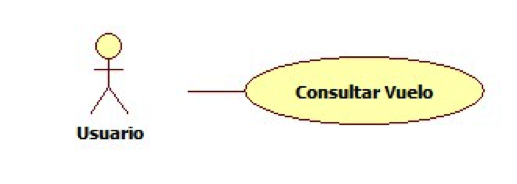
\includegraphics[width=0.9\textwidth]{Figuras/cuConsultarVuelo.png}
		\rule{30em}{0.5pt}
	\caption[Diagrama de Caso de Uso Consultar Vuelo]{Diagrama de Caso de Uso Consultar Vuelo}
	\label{fig:cuConsultarVuelo}
\end{figure}

\begin{longtable}{|p{2.5cm}|p{6.4cm}|p{2cm}|p{2cm}|}
	\hline
		\rowcolor[RGB]{51,153,255}{Caso de Uso}&\multicolumn{2}{c}{Consultar Vuelo}&{\textbf{CU-U-04}}\\
	\hline
		{Actores}&\multicolumn{3}{p{11.2cm}|}{Usuario}\\
	\hline
		{Tipo}&\multicolumn{3}{p{11.2cm}|}{Esencial}\\
	\hline
		{Precondición}&\multicolumn{3}{p{11.2cm}|}{Existen vuelos registrados en el Web Service.}\\
	\hline
		{Postcondición}&\multicolumn{3}{p{11.2cm}|}{El turista tiene a su disposición la información de vuelos acorde a sus posibilidades y configuración de viaje.}\\
	\hline
		{Autor}&{Barajas Uribe Sergio}&{\textbf{Fecha} 06/06/15}&{\textbf{Versión} 3.0}\\
			\hline
		{Evaluador}&{Barajas Uribe Sergio}&{\textbf{Fecha} 08/06/15}&{\textbf{Estatus} Aprobado}\\
	\hline
		{Propósito}&\multicolumn{3}{p{11.2cm}|}{Consultar información de vuelos.}\\
	\hline
		{Resumen}&\multicolumn{3}{p{11.2cm}|}{El usuario realiza una búsqueda de vuelos y se muestra un listado de los mismos según los parámetros de la búsqueda.}\\	
	\hline
		{Comentarios}&\multicolumn{3}{p{11.2cm}|}{Si el usuario ha realizado su configuración, la clase por defecto será la que el configuró.}\\	
	\hline
	\caption[Especificación del Caso de Uso Consultar Vuelo]{Especificación del Caso de Uso Consultar Vuelo}
    	\label{tab:cuConsultarVuelo}
\end{longtable}
\newpage
\begin{flushleft}
	\textbf{Trayectoria Principal}\\
	\begin{enumerate}
		\item El usuario solicita consultar vuelos. \hyperlink{TrayectoriaA_CU-U-04}{[Trayectoria A]}.
		\item Se despliega un formulario para realizar la búsqueda según: origen, destino y clase (Económico, Económico Premium, Business, Primera).
		\item El usuario selecciona los parámetros de interés. \hyperlink{TrayectoriaB_CU-U-04}{[Trayectoria B]}.
		\item Se  muestra un listado de vuelos disponibles con las características requeridas. \hyperlink{TrayectoriaC_CU-U-04}{[Trayectoria C]}.
	\end{enumerate}
\end{flushleft}
----Fin del caso de uso

\begin{flushleft}
	\hypertarget{TrayectoriaA_CU-U-04}{}
	\textbf{Trayectoria Alternativa A}\\
	\textbf{Condición:} La conexión con el servidor se pierde. \\
	\textbf{Nota: } Este curso alterno puede presentarse en cualquier momento durante el curso de CU-U-04. \\	
	\begin{enumerate}
		\item El cliente debe reintentar completar la operación en otro momento. 
		\item Volver a 1. 
	\end{enumerate}
\end{flushleft}
----Fin de Trayectoria

\begin{flushleft}
	\hypertarget{TrayectoriaB_CU-U-04}{}
	\textbf{Trayectoria Alternativa B}\\
	\textbf{Condición:} El usuario no ha ingresado los parámetros adecuados para la búsqueda. \\
	\begin{enumerate}
		\item  Se notifica al usuario y se solicita que indique los parámetros adecuados para la búsqueda.
	\end{enumerate}
\end{flushleft}
----Fin de Trayectoria

\begin{flushleft}
	\hypertarget{TrayectoriaC_CU-U-04}{}
	\textbf{Trayectoria Alternativa C}\\
	\textbf{Condición:} La búsqueda no obtiene resultados con las características requeridas. \\
	\begin{enumerate}
		\item Se despliega una notificación de aviso y se solicita iniciar una nueva búsqueda. 
		\item Volver a 1.
	\end{enumerate}
\end{flushleft}
----Fin de Trayectoria
\clearpage
\subsection{Caso de Uso Consultar Información AICM}

\begin{figure}[htbp]
	\centering
		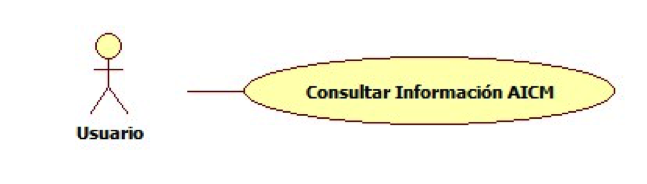
\includegraphics[width=0.9\textwidth]{Figuras/cuConsultarInformacionAICM.png}
		\rule{30em}{0.5pt}
	\caption[Diagrama de Caso de Uso Consultar Informacion AICM]{Diagrama de Caso de Uso Consultar Informacion AICM}
	\label{fig:cuConsultarInformacionAICM}
\end{figure}

\begin{longtable}{|p{2.5cm}|p{6.4cm}|p{2cm}|p{2cm}|}
	\hline
		\rowcolor[RGB]{51,153,255}{Caso de Uso}&\multicolumn{2}{c}{Consultar Información AICM}&{\textbf{CU-U-05}}\\
	\hline
		{Actores}&\multicolumn{3}{p{11.2cm}|}{Usuario}\\
	\hline
		{Tipo}&\multicolumn{3}{p{11.2cm}|}{Esencial}\\
	\hline
		{Precondición}&\multicolumn{3}{p{11.2cm}|}{El administrador ha registrado en el sistema la información del AICM.}\\
	\hline
		{Postcondición}&\multicolumn{3}{p{11.2cm}|}{El usuario tiene a su disposición la información sobre el AICM.}\\
	\hline
		{Autor}&{Vivanco Carmona Erick Rafael}&{\textbf{Fecha} 09/01/15}&{\textbf{Versión} 2.0}\\
			\hline
		{Evaluador}&{Barajas Uribe Sergio}&{\textbf{Fecha} 15/01/15}&{\textbf{Estatus} Aprobado}\\
	\hline
		{Propósito}&\multicolumn{3}{p{11.2cm}|}{Consultar la información relacionada con el AICM como es el teléfono del aeropuerto para consultar alguna duda, ubicación, servicios, mapa y página web.}\\
	\hline
		{Resumen}&\multicolumn{3}{p{11.2cm}|}{El usuario consulta la información del AICM que previamente ha sido registrada por el administrador y se encuentra disponible en la aplicación.}\\	
	\hline
	\caption[Especificación del Caso de Uso Consultar Información AICM]{Especificación del Caso de Uso Consultar Información AICM}
    	\label{tab:cuConsultarInformacionAICM}
\end{longtable}

\begin{flushleft}
	\textbf{Trayectoria Principal}\\
	\begin{enumerate}
		\item El usuario solicita la información del AICM. \hyperlink{TrayectoriaA_CU-U-05}{[Trayectoria A]}.
		\item Se despliega la información del AICM.
	\end{enumerate}
\end{flushleft}
----Fin del caso de uso

\begin{flushleft}
	\hypertarget{TrayectoriaA_CU-U-05}{}
	\textbf{Trayectoria Alternativa A}\\
	\textbf{Condición:} No existe información registrada o disponible en el sistema. \\
	\begin{enumerate}
		\item  Se notifica al turista. 
		\item Termina la operación.
	\end{enumerate}
\end{flushleft}
----Fin de Trayectoria
\clearpage

\subsection{Caso de Uso Gestionar Equipaje}

\begin{figure}[htbp]
	\centering
		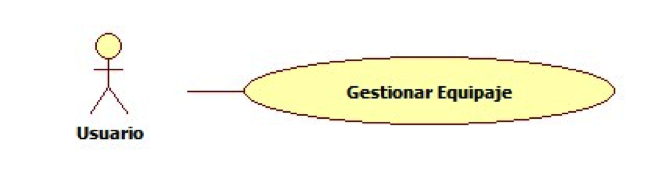
\includegraphics[width=0.9\textwidth]{Figuras/cuGestionarEquipajeU.png}
		\rule{30em}{0.5pt}
	\caption[Diagrama de Caso de Uso Gestionar Equipaje]{Diagrama de Caso de Uso Gestionar Equipaje}
	\label{fig:cuGestionarEquipajeU}
\end{figure}
\begin{longtable}[h!]{|p{2.5cm}|p{6.4cm}|p{2cm}|p{2cm}|}
	\hline
		\rowcolor[RGB]{51,153,255}{Caso de Uso}&\multicolumn{2}{c}{Gestionar Equipaje}&{\textbf{CU-U-06}}\\
	\hline
		{Actores}&\multicolumn{3}{p{11.2cm}|}{Usuario}\\
	\hline
		{Tipo}&\multicolumn{3}{p{11.2cm}|}{Esencial}\\
	\hline
		{Precondición}&\multicolumn{3}{p{11.2cm}|}{El administrador ha registrado objetos de viaje.}\\
	\hline
		{Postcondición}&\multicolumn{3}{p{11.2cm}|}{El usuario tiene a su disposición objetos para crear lista de equipaje.}\\
	\hline
		{Autor}&{Vivanco Carmona Erick Rafael}&{\textbf{Fecha} 09/01/15}&{\textbf{Versión} 2.0}\\
			\hline
		{Evaluador}&{Barajas Uribe Sergio}&{\textbf{Fecha} 15/01/15}&{\textbf{Estatus} Aprobado}\\
	\hline
		{Propósito}&\multicolumn{3}{p{11.2cm}|}{Consultar el equipaje del usuario necesario para su viaje.}\\
	\hline
		{Resumen}&\multicolumn{3}{p{11.2cm}|}{El usuario selecciona objetos dependiendo del tipo de viaje que vaya a realizar y consulta los objetos seleccionados para su comprobación.}\\	
	\hline
		{Comentarios}&\multicolumn{3}{p{11.2cm}|}{Existen equipajes predeterminados, pero el usuario puede crear el suyo personalizado.}\\
	\hline
	\caption[Especificación del Caso de Uso Gestionar Equipaje]{Especificación del Caso de Uso Gestionar Equipaje}
    	\label{tab:cuGestionarEquipajeU}
\end{longtable}

\begin{flushleft}
	\textbf{Trayectoria Principal}\\
	\begin{enumerate}
		\item El usuario solicita crear lista de equipaje.
		\item Se solicita el nombre de la categoría de viaje.
		\item Se solicita los objetos requeridos para la lista de equipaje.
		\item Se crea la lista de equipaje.
		\item El usuario solicita verificar su equipaje.
		\item Se despliegan los objetos registrados en la lista de equipaje.
		\item El usuario verifica los objetos.
		\item El usuario edita lista de equipaje.
		\item El usuario añade objetos a la lista de equipaje.
	\end{enumerate}
\end{flushleft}
----Fin del caso de uso
\clearpage

\subsection{Caso de Uso Consultar Itinerario de Viaje}
\hypertarget{CU-U-07}{}

\begin{figure}[htbp]
	\centering
		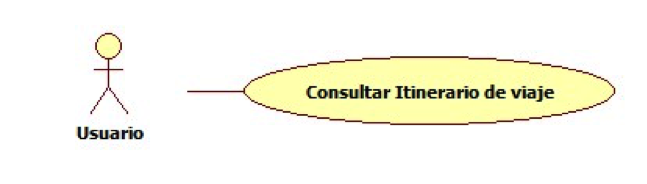
\includegraphics[width=0.9\textwidth]{Figuras/cuConsultarItinerarioViaje.png}
		\rule{30em}{0.5pt}
	\caption[Diagrama de Caso de Uso Consultar Itinerario de Viaje]{Diagrama de Caso de Uso Consultar Itinerario de Viaje}
	\label{fig:cuConsultarItinerarioViaje}
\end{figure}

\begin{longtable}{|p{2.5cm}|p{6.4cm}|p{2cm}|p{2cm}|}
	\hline
		\rowcolor[RGB]{51,153,255}{Caso de Uso}&\multicolumn{2}{c}{Consultar Itinerario de Viaje}&{\textbf{CU-U-07}}\\
	\hline
		{Actores}&\multicolumn{3}{p{11.2cm}|}{Usuario}\\
	\hline
		{Tipo}&\multicolumn{3}{p{11.2cm}|}{Esencial}\\
	\hline
		{Precondición}&\multicolumn{3}{p{11.2cm}|}{El usuario debe registrar una lista de actividades que realizará en el viaje.}\\
	\hline
		{Postcondición}&\multicolumn{3}{p{11.2cm}|}{El usuario tiene a su disposición un itinerario de su viaje con las posibles 
		actividades a realizar en el mismo.}\\
	\hline
		{Autor}&{Vivanco Carmona Erick Rafael}&{\textbf{Fecha} 09/01/15}&{\textbf{Versión} 2.0}\\
			\hline
		{Evaluador}&{Barajas Uribe Sergio}&{\textbf{Fecha} 15/01/15}&{\textbf{Estatus} Aprobado}\\
	\hline
		{Propósito}&\multicolumn{3}{p{11.2cm}|}{Atender las distintas actividades que se ha planteado el propio usuario en su viaje en proceso.}\\
	\hline
		{Resumen}&\multicolumn{3}{p{11.2cm}|}{El usuario obtiene la información de su itinerario de viaje que haya descrito previamente.}\\	
	\hline
		{Comentarios}&\multicolumn{3}{p{11.2cm}|}{El itinerario que se muestre será a partir de las actividades que el usuario ingrese.}\\	
	\hline
	\caption[Especificación del Caso de Uso Consultar Itinerario de Viaje]{Especificación del Caso de Uso Consultar Itinerario de Viaje}
    	\label{tab:cuConsultarItinerarioViaje}
\end{longtable}
\newpage
\begin{flushleft}
	\textbf{Trayectoria Principal}\\
	\begin{enumerate}
		\item El usuario solicita itinerario de viaje.
		\item El sistema solicita una lista de actividades que el usuario gusta realizar en su viaje (itinerario).
		\item Se despliega actividades para viaje.
		\item El usuario puede gestionar su itinerario modificando, agregando o eliminando actividades.
	\end{enumerate}
\end{flushleft}
----Fin del caso de uso

\begin{flushleft}
	\hypertarget{TrayectoriaA_CU-U-07}{}
	\textbf{Trayectoria Alternativa A}\\
	\textbf{Condición:} El usuario no ha registrado itinerario\\
	\begin{enumerate}
		\item El usuario no puede consultar itinerario si aun no ha registrado alguno.
	\end{enumerate}
\end{flushleft}
----Fin de Trayectoria

\begin{flushleft}
	\hypertarget{TrayectoriaB_CU-U-07}{}
	\textbf{Trayectoria Alternativa B}\\
	\textbf{Condición:} La conexión con el servidor se pierde. \\
	\begin{enumerate}
		\item Los datos del vuelo no pueden ser cargados correctamente. 
		\item El cliente debe reintentar completar la operación en otro momento. 
		\item Volver a 2. 
	\end{enumerate}
\end{flushleft}
----Fin de Trayectoria
\clearpage

\subsection{Caso de Uso Consultar Ruta casa-AICM}

\begin{figure}[htbp]
	\centering
		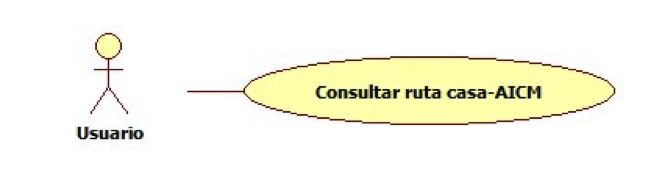
\includegraphics[width=0.9\textwidth]{Figuras/cuConsultarRutacasa-AICM.png}
		\rule{30em}{0.5pt}
	\caption[Diagrama de Caso de Uso Consultar Ruta casa-AICM]{Diagrama de Caso de Uso Consultar Ruta casa-AICM}
	\label{fig:cuConsultarRutacasa-AICM}
\end{figure}

\begin{longtable}{|p{2.5cm}|p{6.4cm}|p{2cm}|p{2cm}|}
	\hline
		\rowcolor[RGB]{51,153,255}{Caso de Uso}&\multicolumn{2}{c}{Consultar Ruta casa-AICM}&{\textbf{CU-U-08}}\\
	\hline
		{Actores}&\multicolumn{3}{p{11.2cm}|}{Usuario}\\
	\hline
		{Tipo}&\multicolumn{3}{p{11.2cm}|}{Esencial}\\
	\hline
		{Precondición}&\multicolumn{3}{p{11.2cm}|}{El usuario deberá estar conectado a una red de internet para generar la ruta de su origen al aeropuerto.}\\
	\hline
		{Postcondición}&\multicolumn{3}{p{11.2cm}|}{Se obtiene la ruta desde el punto de origen hacia el AICM.}\\
	\hline
		{Autor}&{Vivanco Carmona Erick Rafael}&{\textbf{Fecha} 09/01/15}&{\textbf{Versión} 2.0}\\
			\hline
		{Evaluador}&{Barajas Uribe Sergio}&{\textbf{Fecha} 15/01/15}&{\textbf{Estatus} Aprobado}\\
	\hline
		{Propósito}&\multicolumn{3}{p{11.2cm}|}{Obtener la ruta desde el origen del usuario al AICM.}\\
	\hline
		{Resumen}&\multicolumn{3}{p{11.2cm}|}{El usuario desea conocer cuál es la ruta para llegar al AICM desde su punto de origen. Por lo tanto, solicita dicha función al sistema, el sistema obtiene la ubicación actual del usuario y  genera la ruta hacia el AICM.}\\	
	\hline
		{Comentarios}&\multicolumn{3}{p{11.2cm}|}{El usuario debe estar conectado a una red para generar la ruta.}\\
	\hline
	\caption[Especificación del Caso de Uso Consultar Ruta casa-AICM]{Especificación del Caso de Uso Consultar Ruta casa-AICM}
    	\label{tab:cuConsultarRutacasa-AICM}
\end{longtable}
\clearpage

\begin{flushleft}
	\textbf{Trayectoria Principal}\\
	\begin{enumerate}
		\item El usuario solicita generar una nueva ruta hacia el AICM. \hyperlink{TrayectoriaA_CU-U-08}{[Trayectoria A]}.
		\item Se obtiene la ubicación actual del usuario.
		 item Se pone el primer marcador a la ubicación actual y un segundo en la ubicación destino posteriormente se genera la ruta hacia el AICM
		\item El usuario tiene a su disposición la ruta sugerida por el sistema para llegar desde su ubicación actual hacia el AICM.
	\end{enumerate}
\end{flushleft}
----Fin del caso de uso

\begin{flushleft}
	\hypertarget{TrayectoriaA_CU-U-08}{}
	\textbf{Trayectoria Alternativa A}\\
	\textbf{Condición:} No existe conexión con una red para generar la ruta. \\
	\begin{enumerate}
		\item Se solicita al usuario que se conecte a una red para generar la ruta. 
		\item Volver a 1.
	\end{enumerate}
\end{flushleft}
----Fin de Trayectoria
\clearpage

\subsection{Caso de Uso Ubicar en AICM}

\begin{figure}[htbp]
	\centering
		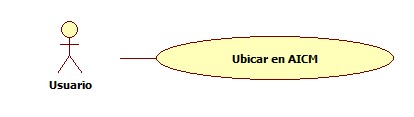
\includegraphics[width=0.9\textwidth]{Figuras/cuUbicarAICM.jpg}
		\rule{30em}{0.5pt}
	\caption[Diagrama de Caso de Uso Ubicar en AICM]{Diagrama de Caso de Uso Ubicar en AICM}
	\label{fig:cuUbicarAICM}
\end{figure}

\begin{longtable}{|p{2.5cm}|p{6.4cm}|p{2cm}|p{2cm}|}
	\hline
		\rowcolor[RGB]{51,153,255}{Caso de Uso}&\multicolumn{2}{c}{Ubicar en AICM}&{\textbf{CU-U-09}}\\
	\hline
		{Actores}&\multicolumn{3}{p{11.2cm}|}{Usuario}\\
	\hline
		{Tipo}&\multicolumn{3}{p{11.2cm}|}{Esencial}\\
	\hline
		{Precondición}&\multicolumn{3}{p{11.2cm}|}{El sistema deberá estar entrenado en el AICM.}\\
	\hline
		{Postcondición}&\multicolumn{3}{p{11.2cm}|}{Se obtiene la localización del usuario dentro del AICM.}\\
	\hline
		{Autor}&{Vivanco Carmona Erick Rafael}&{\textbf{Fecha} 09/01/15}&{\textbf{Versión} 2.0}\\
			\hline
		{Evaluador}&{Barajas Uribe Sergio}&{\textbf{Fecha} 15/01/15}&{\textbf{Estatus} Aprobado}\\
	\hline
		{Propósito}&\multicolumn{3}{p{11.2cm}|}{Obtener la ubicación del usuario dentro del AICM mediante el magnetómetro integrado en el dispositivo móvil. }\\
	\hline
		{Resumen}&\multicolumn{3}{p{11.2cm}|}{El usuario solicita explorar el AICM, el sistema despliega el mapa del AICM-T1 para facilitar la localización dentro del mismo.}\\	
	\hline
		{Comentarios}&\multicolumn{3}{p{11.2cm}|}{El sistema deberá estar entrenado, de lo contrario, la ubicación será ineficiente.}\\
	\hline
	\caption[Especificación del Caso de Uso Ubicar en AICM]{Especificación del Caso de Uso Ubicar en AICM}
    	\label{tab:cuUbicarAICM}
\end{longtable}
\clearpage

\begin{flushleft}
	\textbf{Trayectoria Principal}\\
	\begin{enumerate}
		\item El usuario solicita localizarse en el AICM.
		\item El sistema despliega un mapa del AICM donde se puede ubicar al usuario así como las distintas salas de abordaje con las que cuenta el 
		aeropuerto.
		\item El usuario tiene a su disposición el mapa el cual le mostrará su ubicación actual.
	\end{enumerate}
\end{flushleft}
----Fin del caso de uso
\clearpage

\subsection{Caso de Uso Consultar Información de Vuelo}

\begin{figure}[htbp]
	\centering
		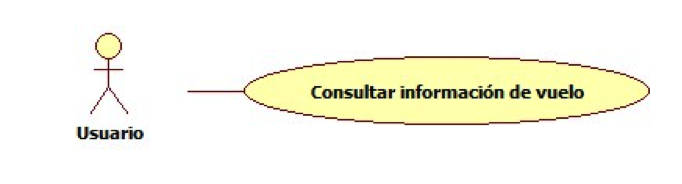
\includegraphics[width=0.9\textwidth]{Figuras/cuConsultarInformacionVuelo.png}
		\rule{30em}{0.5pt}
	\caption[Diagrama de Caso de Uso Consultar Información de Vuelo]{Diagrama de Caso de Uso Consultar Información de Vuelo}
	\label{fig:cuConsultarInformacionVuelo}
\end{figure}

\begin{longtable}{|p{2.5cm}|p{6.4cm}|p{2cm}|p{2cm}|}
	\hline
		\rowcolor[RGB]{51,153,255}{Caso de Uso}&\multicolumn{2}{c}{Consultar Información de Vuelo}&{\textbf{CU-U-10}}\\
	\hline
		{Actores}&\multicolumn{3}{p{11.2cm}|}{Usuario}\\
	\hline
		{Tipo}&\multicolumn{3}{p{11.2cm}|}{Esencial}\\
	\hline
		{Precondición}&\multicolumn{3}{p{11.2cm}|}{El usuario ha ingresado su número de vuelo.}\\
	\hline
		{Postcondición}&\multicolumn{3}{p{11.2cm}|}{El usuario tendrá a su disposición la información de su vuelo.}\\
	\hline
		{Autor}&{Vivanco Carmona Erick Rafael}&{\textbf{Fecha} 09/01/15}&{\textbf{Versión} 2.0}\\
			\hline
		{Evaluador}&{Barajas Uribe Sergio}&{\textbf{Fecha} 15/01/15}&{\textbf{Estatus} Aprobado}\\
	\hline
		{Propósito}&\multicolumn{3}{p{11.2cm}|}{Consultar la información relacionada con el vuelo del usuario.}\\
	\hline
		{Resumen}&\multicolumn{3}{p{11.2cm}|}{El usuario solicita la información relacionada con un número de vuelo específico. Una vez ingresado el número de vuelo el sistema proporciona el estado del vuelo, la ciudad de origen, hora de salida, terminal y puerta.}\\	
	\hline
	\caption[Especificación del Caso de Uso Consultar Información de Vuelo]{Especificación del Caso de Uso Consultar Información de Vuelo}
    	\label{tab:cuConsultarInformacionVuelo}
\end{longtable}

\begin{flushleft}
	\textbf{Trayectoria Principal}\\
	\begin{enumerate}
		\item El usuario tiene a sus disposición información referente a vuelos en curso, separados por salidas y llegadas, tanto Nacionales 
		como Internacionales.
		\item El usuario solicita la información de vuelo. \hyperlink{TrayectoriaA_CU-U-10}{[Trayectoria A]}.
		\item El sistema solicita el número de vuelo.
		\item El sistema despliega la información relacionada con el número de vuelo. \hyperlink{TrayectoriaB_CU-U-10}{[Trayectoria B]} \hyperlink{TrayectoriaC_CU-U-10}{[Trayectoria C]}.
		\item El usuario tiene a su disposición la información referente a su vuelo.
	\end{enumerate}
\end{flushleft}
----Fin del caso de uso

\begin{flushleft}
	\hypertarget{TrayectoriaA_CU-U-10}{}
	\textbf{Trayectoria Alternativa A}\\
	\textbf{Condición:} Solicitar información del vuelo \\
	\begin{enumerate}
		\item Se notifica al usuario si existe un número de vuelo registrado.
		\item Se continúa con el proceso.
	\end{enumerate}
\end{flushleft}
----Fin de Trayectoria

\begin{flushleft}
	\hypertarget{TrayectoriaB_CU-U-10}{}
	\textbf{Trayectoria Alternativa B}\\
	\textbf{Condición:} La conexión con el servidor se pierde. \\
	\begin{enumerate}
		\item Los datos del vuelo no pueden ser cargados correctamente. 
		\item El cliente debe reintentar completar la operación en otro momento. 
		\item Volver a 1.
	\end{enumerate}
\end{flushleft}
----Fin de Trayectoria

\begin{flushleft}
	\hypertarget{TrayectoriaC_CU-U-10}{}
	\textbf{Trayectoria Alternativa C}\\
	\textbf{Condición:} La conexión con la red se pierde. \\
	\begin{enumerate}
		\item El cliente debe reintentar completar la operación en otro momento. 
		\item Volver a 1.
	\end{enumerate}
\end{flushleft}
----Fin de Trayectoria
\newpage